

\section{Course 1 Week 1. Introduction to deep learning} 

\paragraph{}
In this week, questions such as,\newline
* "Why did neural network become popular?"\newline
are answered.

\subsection{Why is deep learning taking off?} Data-driven solving, so-called problem solving by machine learning, is actually not a new concept at all. Moreover, the theoretical performance of large neural network based machine learning method has been well known to researchers for decades. 
\begin{figure}[H]
\centering
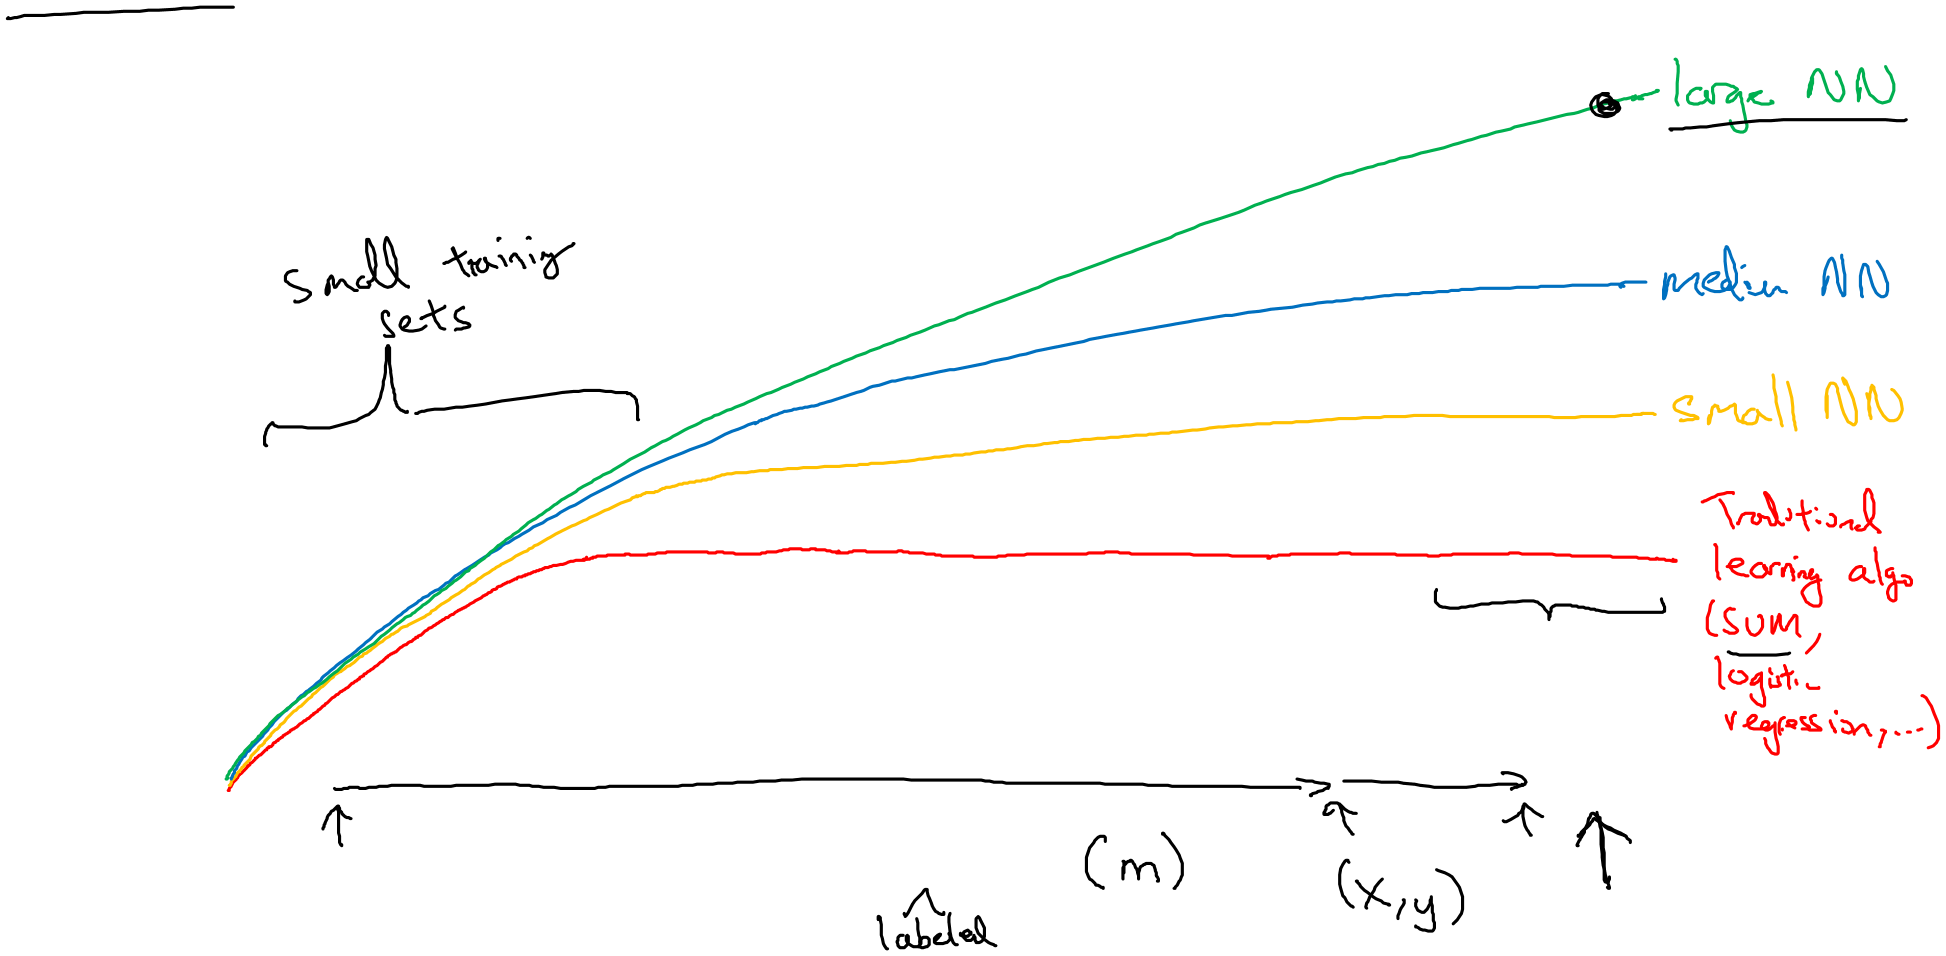
\includegraphics[height=6.2cm]{c1w1_pic1.png}
\caption{For many real world supervised learning problems, performance of large neural networks outperforms many other cases when data size is sufficiently big.}
\end{figure}

Large neural networks, however, could only recently reach its theoretical performance level thanks to the following reasons : 

\paragraph{Digitization of the society and big data} Over the last 20 years, digitization of everything, i.e. work of turning all kinds of information into 0s and 1s, has enabled a incredibly cheaper access to large set of data. 

\paragraph{Computation speed} The circle in figure 2 illustrates the standard procedure of machine learning approaches. How fast one can iterate this procedure determines the feasibility of a machine learning method in the real world problems. Few years before now, the experiment phase of large neural networks was considered too slow to be implemented. Nowadays, the recent enormous advances in computation speed thanks to hardware technologies and algorithm technologies has made experiment phase of large neural network methods feasible.
\begin{figure}[H]
\centering

\includegraphics[height=6.2cm]{c1w1_pic2.png}
\caption{Iteration speed of one circle became fast enough to make large neural net successfully implemented.}
\end{figure}


\subsection{Why is deep learning taking off?}